\documentclass[letterpaper,10pt]{article}

\usepackage{amsmath,amssymb,amsfonts}
\usepackage{algorithmic}
\usepackage{algorithm}
\usepackage{graphicx}
\usepackage{textcomp}
\usepackage{xcolor}
\usepackage{booktabs}
\usepackage{hyperref}
\usepackage{subcaption}
\usepackage{multirow}
\usepackage{cite}
\usepackage[margin=1in]{geometry}
\usepackage{titling}
\usepackage{titlesec}
\usepackage{times}
\tolerance=2000
\hyphenpenalty=1000
\emergencystretch=1em
\usepackage{indentfirst}

\titleformat{\section}{\large\bfseries}{\thesection}{1em}{}
\titleformat{\subsection}{\normalsize\bfseries}{\thesubsection}{1em}{}

\setlength{\droptitle}{-2em}

\begin{document}

\title{\textbf{\Large Semantic-Aware Resource Scheduling on Clusters}}

\author{
Krish Chaudhary \\
\textit{University of Pennsylvania} \\
krish@seas.upenn.edu
}

\date{May 8, 2026}

\twocolumn[
\maketitle

\begin{abstract}
\noindent
Modern GPU clusters run diverse deep learning workloads that exhibit widely varying multi-GPU scaling behavior. Yet, conventional schedulers like SLURM require users to manually specify the number of GPUs for each job---a decision that most researchers and scientists make with little knowledge of their workload's actual scaling characteristics. Users routinely over-provision (wasting resources) or under-provision (leaving performance on the table), and no individual user has the global view needed to optimize cluster-wide throughput. We present a semantic-aware scheduling system that removes this burden entirely: it predicts each job's GPU scaling exponent directly from its training script source code---without requiring any profiling runs---and uses this prediction to automatically make GPU allocation decisions that maximize cluster throughput. Our system employs a large language model to extract model architecture features (family, parameter count, batch size) from submitted scripts, feeds these into a trained regression model to predict the scaling exponent $k$, and applies a greedy marginal-gain allocator to distribute GPUs across concurrent jobs. We evaluate our scheduler against four scheduling algorithms (greedy, polite, FCFS-split, and size-aware) on a cluster of 8 NVIDIA RTX 3060 GPUs across 21 diverse training workloads spanning CNNs, transformers, GANs, GNNs, reinforcement learning, and diffusion models. Our results demonstrate that semantic-aware allocation reduces makespan by up to 40\% compared to naive scheduling algorithms while improving GPU utilization and fairness.
\end{abstract}
\vspace{1em}
]

% ---------------------------------------------------------------------------
\section{Introduction}
\label{sec:introduction}

GPU clusters have become the backbone of modern deep learning research and production training. Organizations invest heavily in multi-GPU nodes, yet analysis of large-scale production clusters shows that nearly 48\% of allocated GPU cycles are wasted, with average utilization across all jobs at only 52\%~\cite{jeon2019analysis}. A key contributor to this underutilization is that \textit{users are expected to choose how many GPUs their jobs need}---a decision they are fundamentally ill-equipped to make.

In practice, a researcher submitting a training job to SLURM must specify a GPU count in their \texttt{sbatch} script. This decision is typically made with no knowledge of the job's actual scaling behavior, no visibility into what other jobs are competing for resources, and no understanding of how their choice affects cluster-wide throughput. The result is predictable: some users over-provision, requesting all available GPUs for a model that barely benefits from a fraction of them, while others under-provision, running a highly parallelizable workload on a single GPU for hours when additional accelerators would have finished it in minutes. Neither user has done anything wrong---the system simply asks them a question they cannot answer.

Current cluster managers such as SLURM compound this problem by requiring explicit GPU requests: if a user omits the \texttt{--gres=gpu:N} flag from their submission, SLURM allocates \textit{zero} GPUs---the job runs on CPU only, regardless of whether GPUs are available. There is no mechanism to automatically determine an appropriate GPU count. Furthermore, SLURM's scheduling policies---FIFO, backfill, and fair-share---treat all GPU requests as equally valid. A user requesting 8 GPUs for a small CNN receives the same treatment as one training a large transformer, despite the fact that these workloads scale very differently with additional GPUs. The CNN may achieve near-linear speedup ($k \approx 0.9$), while the transformer's communication overhead limits its scaling exponent to $k \approx 0.5$, meaning half the allocated GPUs contribute minimal speedup. No amount of user education can fix this: even an expert cannot optimize their own GPU request without knowing the current cluster load and the scaling characteristics of every other queued job.

Our key insight is that a job's GPU scaling efficiency can be predicted \textit{before execution} by analyzing the structure of its training script, and that this prediction should be made by the \textit{scheduler}, not the user. Model architecture, parameter count, and batch size are strong predictors of how well a distributed training job will utilize additional GPUs. By extracting these features automatically and predicting the scaling exponent $k$, the scheduler can make globally-informed allocation decisions: giving more GPUs to jobs that benefit from them, fewer to jobs that would waste them, and removing the GPU-count decision from users entirely.

We present a semantic-aware GPU scheduler that operates as a SLURM overlay. Users submit training scripts without specifying GPU counts. Our system consists of three components: (1) an LLM-based feature extractor that reads submitted training scripts and identifies model family, batch size, and parameter count; (2) a trained regression model that predicts the scaling exponent $k$ from these features; and (3) a greedy marginal-gain allocator that distributes available GPUs across queued jobs to maximize total cluster throughput.

Our contributions are:
\begin{itemize}
    \item A method for predicting GPU scaling efficiency from training script source code without profiling runs.
    \item A greedy GPU allocation algorithm based on marginal speedup gain that accounts for diminishing returns.
    \item A benchmark dataset of 196 DDP training configurations across 57 model families with measured scaling curves.
    \item An evaluation framework that measures scheduler performance across varying levels of cluster contention (3, 5, 12, and 22 concurrent jobs) and inter-arrival delays, comparing against four scheduling algorithms.
\end{itemize}

% ---------------------------------------------------------------------------
\section{Background and Related Work}
\label{sec:related}

\subsection{GPU Cluster Scheduling}

Traditional HPC schedulers like SLURM~\cite{yoo2003slurm} manage job queues using policies such as first-in-first-out (FIFO), backfill scheduling, and priority-based fair-share. These policies are designed for general-purpose workloads and do not consider the GPU scaling characteristics of individual jobs. Users specify GPU requirements manually, often over-provisioning to ensure fast completion.

Kubernetes-based schedulers offer more flexibility through custom resource scheduling, but the dominant paradigm remains static allocation: a job requests $N$ GPUs and keeps them until completion, regardless of whether it effectively utilizes them.

\subsection{Scaling-Aware Schedulers}

Several recent systems have addressed scaling-aware scheduling for deep learning clusters.

Pollux~\cite{pollux2021} jointly optimizes GPU allocation and batch size by modeling a goodput function that accounts for both throughput scaling and statistical efficiency. It dynamically resizes running jobs, adding or removing GPUs based on cluster-wide goodput optimization. However, Pollux requires Kubernetes, elastic training support via AdaptDL, and runtime instrumentation of training scripts.

Optimus~\cite{optimus2018} fits an online performance model by observing job throughput at different GPU counts during execution. It uses these models to allocate resources that minimize average job completion time. Like Pollux, it requires runtime profiling data that is unavailable before a job starts.

Tiresias~\cite{tiresias2019} applies the Least Attained Service (LAS) discipline to GPU scheduling, prioritizing jobs that have consumed fewer GPU-hours. It uses a two-level priority queue with a discretized threshold to prevent long jobs from starving short ones. However, its key mechanism---preemption---requires checkpoint-restart support that many training frameworks lack.

Gandiva~\cite{gandiva2018} exploits intra-job predictability through time-slicing and migration, packing multiple jobs onto the same GPUs through fine-grained sharing. This approach is orthogonal to allocation-level scheduling.

Gavel~\cite{gavel2020} addresses heterogeneity-aware scheduling, optimizing which \textit{type} of GPU to assign to each job (e.g., V100 vs.\ A100) rather than how many. While complementary to our work, Gavel does not address the GPU count allocation problem.

Our system differs from all of these in a fundamental way: we predict scaling behavior \textit{before execution} from source code analysis, enabling informed allocation decisions without runtime profiling, elastic resizing, or preemption. This eliminates a class of costly runtime operations that these systems rely on. Elastic resizing requires checkpointing model state, redistributing data shards, reinitializing communication groups, and reloading optimizer state across a new GPU topology---a process that can take minutes for large models and introduces non-trivial failure modes (e.g., inconsistent checkpoint state, NCCL group reconstruction failures). Preemption-based systems like Tiresias face similar overhead: suspending a multi-GPU training job requires flushing GPU memory, serializing model parameters, and later deserializing them onto potentially different devices. By making the allocation decision \textit{once}, before the job starts, our approach avoids this thrashing entirely. This makes our system compatible with existing SLURM-based clusters without infrastructure changes, and eliminates the risk of mid-training disruptions that can corrupt model convergence or waste GPU cycles on repeated warm-up iterations.

\subsection{Multi-GPU Scaling Behavior}

Distributed data-parallel (DDP) training replicates the model across $g$ GPUs, partitions each mini-batch into $g$ shards, computes gradients independently, and synchronizes via all-reduce before each parameter update. The training time with $g$ GPUs can be modeled as a power law:
\begin{equation}
    T(g) = a \cdot g^{-k}
    \label{eq:scaling}
\end{equation}
where $a$ is the single-GPU baseline time and $k \in [0, 1]$ is the scaling exponent. This model arises from the observation that adding GPUs provides diminishing returns: each additional GPU reduces the per-GPU data shard (improving throughput) but adds communication overhead for gradient synchronization (reducing efficiency).

The exponent $k$ captures the net effect. When $k = 1$, doubling the GPUs halves the training time---perfect linear scaling. In practice, $k < 1$ because:
\begin{itemize}
    \item \textit{All-reduce volume}: gradient synchronization transfers $O(P)$ bytes per iteration, where $P$ is the parameter count. Larger models incur higher communication cost relative to computation.
    \item \textit{Communication-to-computation ratio}: architectures with frequent synchronization points (e.g., transformers with many attention layers) spend more time waiting for gradient aggregation than architectures with large, independent computation blocks (e.g., CNNs with deep convolutional stacks).
    \item \textit{Batch size effects}: DDP effectively multiplies the batch size by $g$. For small per-GPU batch sizes, GPU utilization drops because the hardware is underutilized; for very large effective batch sizes, gradient noise decreases and more iterations may be needed to converge.
    \item \textit{Memory bandwidth}: some operations are memory-bound rather than compute-bound, and adding GPUs does not alleviate memory bandwidth bottlenecks within each device.
\end{itemize}

The power-law model fits empirical scaling data well: in our benchmark of 196 configurations, 189 achieve $R^2 > 0.9$ when fitting $\log T(g) = \log a - k \cdot \log g$ by linear regression. This validates the choice of a single-parameter scaling model over more complex alternatives.

Crucially, $k$ depends on \textit{architectural} factors---model structure, layer types, parameter count, and batch size---rather than \textit{data} factors like dataset size or number of epochs. The latter affect only the constant $a$ (scaling total iterations linearly) without changing the relative speedup from additional GPUs. This separation means $k$ can be predicted from static analysis of the training script's source code, without needing to observe the job at runtime.

% ---------------------------------------------------------------------------
\section{System Design}
\label{sec:design}

\subsection{Overview}

Our system operates as a user-space overlay on top of SLURM. Figure~\ref{fig:architecture} shows the pipeline: when a user submits a training script, the system (1) extracts model features via an LLM, (2) predicts the scaling exponent $k$, (3) queues the job with its predicted $k$, and (4) allocates GPUs using a greedy marginal-gain algorithm when resources become available. Additionally, the system implements a \textit{continuous retraining pipeline}: when each job completes, its actual runtime, throughput, and GPU utilization metrics are parsed from the job output and appended to the benchmark dataset. This allows the $k$-predictor to be periodically retrained on an expanding corpus that includes real workloads observed in production, improving prediction accuracy over time as the system encounters new model architectures and training configurations.

\begin{figure*}[t]
    \centering
    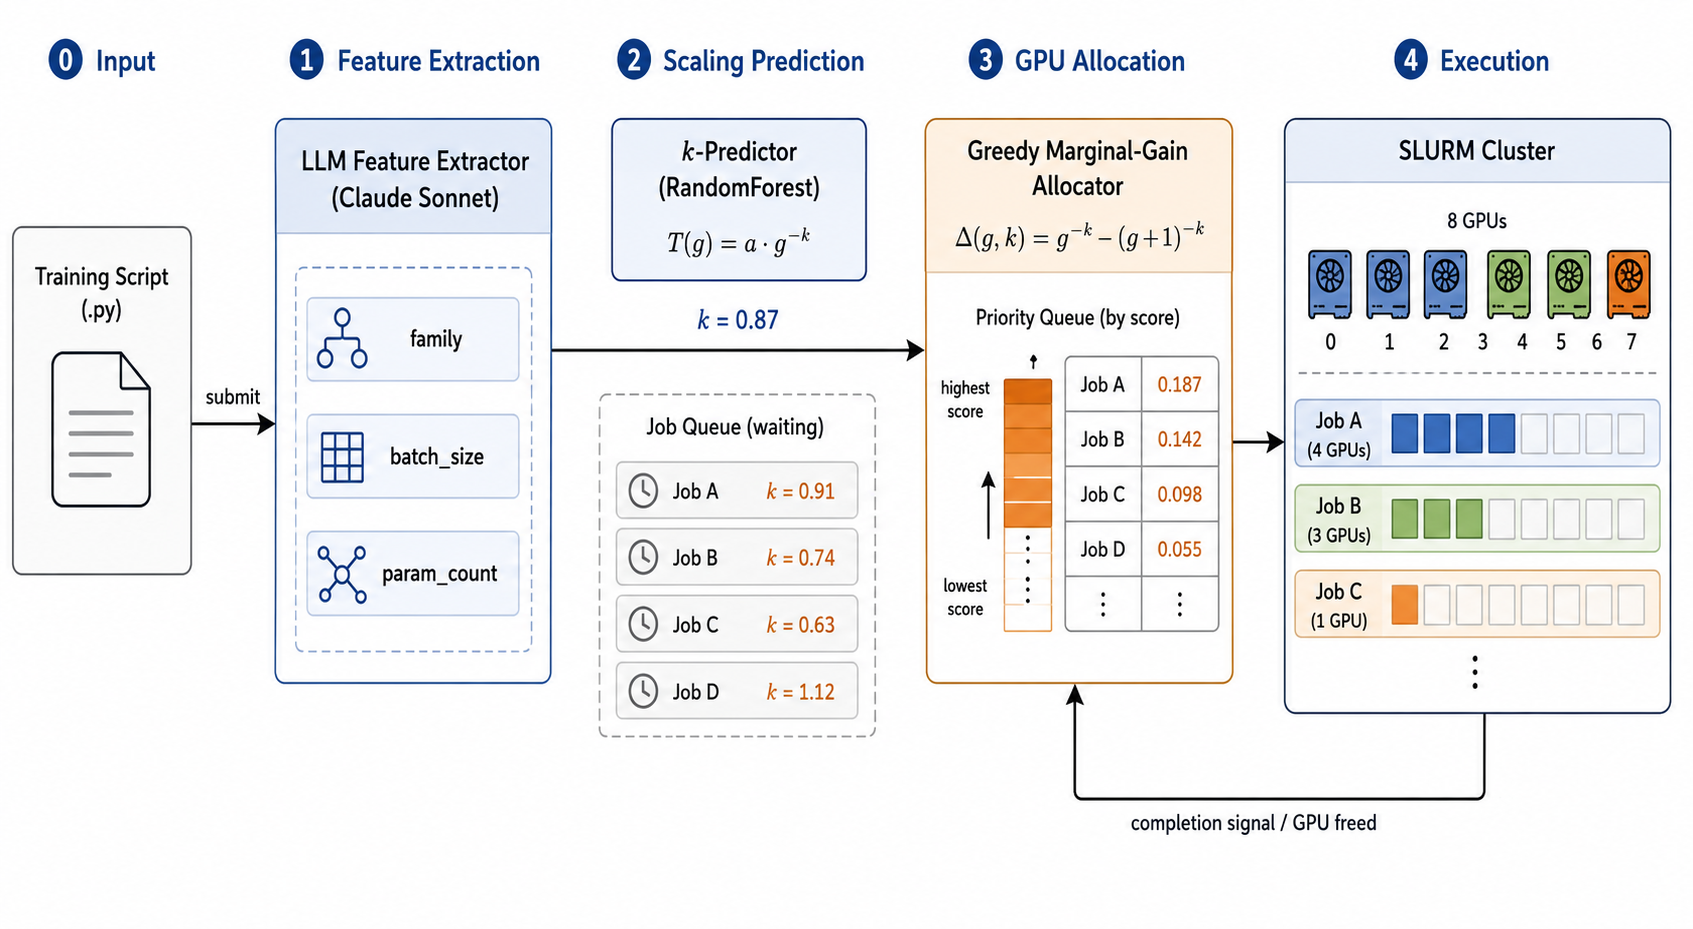
\includegraphics[width=\textwidth]{system_design.png}
    \caption{System architecture of the semantic-aware GPU scheduler. A submitted training script is analyzed by an LLM to extract model features (family, batch size, parameter count), which are fed into a trained RandomForest regressor to predict the scaling exponent $k$. Jobs are queued with their predicted $k$ values and scored by marginal speedup gain $\Delta(g, k) = g^{-k} - (g+1)^{-k}$. The greedy allocator distributes available GPUs one at a time to the highest-scoring job, then submits the allocation to SLURM. A completion signal feeds back to the allocator when GPUs are freed.}
    \label{fig:architecture}
\end{figure*}

\subsection{Benchmark Data Collection}

We constructed a benchmark corpus of 196 PyTorch DDP training scripts spanning 57 model families organized into 13 categories: CNN, ResNet, Transformer, Diffusion, GNN, GAN, Recommender, Audio, Video, Reinforcement Learning, Multi-Modal, MLP, and Other. All model architectures were sourced from the PyTorch Benchmark suite\footnote{\url{https://github.com/pytorch/benchmark}} and adapted for distributed data-parallel training with NCCL, synthetic datasets, and the standardized output protocol required by our benchmark runner.

For each model family, we created four configurations by varying two axes: batch size (small and large) and parameter count (small and large). For example, AlexNet has configurations \texttt{alexnet\_32\_small}, \texttt{alexnet\_32\_large}, \texttt{alexnet\_128\_small}, and \texttt{alexnet\_128\_large}, where the first number denotes batch size and the suffix denotes model size. This $2 \times 2$ design captures how both batch size and model capacity independently affect GPU scaling behavior, providing the predictor with diverse training signal within each architecture family.

Each configuration was benchmarked at GPU counts $\{1, 2, 4, 8\}$ on a single node. After excluding failed runs and incomplete configurations, we retained 196 configurations across 787 total training runs. For each run, we measured total training time, average throughput, peak VRAM usage, SM utilization, and memory bandwidth utilization. All scripts use synthetic datasets to eliminate I/O variability and ensure reproducibility across runs.

\subsection{Fitting the Scaling Exponent}

Given the benchmark measurements $\{(g_i, T_i)\}$ for each configuration, we fit the scaling exponent $k$ from Equation~\ref{eq:scaling} by applying a log transformation to both sides:
\begin{equation}
    \log T(g) = \log a - k \cdot \log g
\end{equation}
This linearizes the power-law relationship: plotting $\log T$ against $\log g$ yields a line with slope $-k$ and intercept $\log a$. We fit this line using ordinary least-squares regression on the four data points ($g \in \{1, 2, 4, 8\}$) for each configuration.

The goodness of fit ($R^2$) indicates how well the power-law model describes each workload's scaling behavior. Configurations where the relationship is non-monotonic (e.g., training time increases with more GPUs due to excessive communication overhead) or noisy produce low $R^2$ values. We filter configurations with $R^2 < 0.9$, retaining 189 configurations across 50 unique models. The resulting $k$ values range from 0.3 (poor scaling, e.g., small GNNs with high communication-to-computation ratios) to 1.0+ (near-perfect or super-linear scaling, e.g., memory-bound workloads that benefit from distributed caching).

Each retained configuration produces one training example for the predictor: the input features are (batch size, parameter count, model family) and the target is the fitted $k$. This dataset forms the basis for learning to predict $k$ from static features alone.

\subsection{Scaling Exponent Predictor}

We train a regression model to predict $k$ from three features: batch size, parameter count, and model family (one-hot encoded across 13 categories). We compared four model families:

\begin{table}[h]
\centering
\caption{5-fold GroupKFold CV losses for $k$ prediction}
\label{tab:cv_results}
\begin{tabular}{lcc}
\toprule
Model & MAE & RMSE \\
\midrule
Ridge & 0.1342 $\pm$ 0.016 & 0.1660 $\pm$ 0.025 \\
RandomForest & \textbf{0.1063} $\pm$ 0.015 & \textbf{0.1341} $\pm$ 0.020 \\
GradBoosting & 0.1126 $\pm$ 0.016 & 0.1441 $\pm$ 0.025 \\
MLP & 0.1541 $\pm$ 0.035 & 0.2019 $\pm$ 0.053 \\
\midrule
Predict-mean & 0.1256 $\pm$ 0.009 & 0.1497 $\pm$ 0.008 \\
\bottomrule
\end{tabular}
\end{table}

GroupKFold cross-validation ensures that all configurations of the same model appear in the same fold, preventing leakage. The RandomForest regressor achieves the best MAE of 0.1063, significantly below the predict-mean baseline of 0.1256.

We note that these prediction results reflect limited GPU wall time available for benchmark data collection. Each of the 196 configurations was benchmarked at only four GPU counts $\{1, 2, 4, 8\}$ with a single run per configuration, providing relatively sparse scaling curves for fitting $k$. With additional GPU time, the benchmark corpus could be expanded in several ways that would directly improve prediction accuracy: (1)~more GPU counts per configuration (e.g., 3, 5, 6, 7) to produce denser scaling curves with tighter $R^2$ fits; (2)~multiple runs per configuration to reduce measurement noise; and (3)~additional model families and configurations to expand training set coverage. We expect that even modest increases in benchmarking budget would yield meaningful improvements in MAE, as the current predictor already outperforms the mean baseline with limited data. Notably, the MLP regressor (MAE 0.1541) underperforms even the predict-mean baseline---a result we attribute entirely to the small training set size (189 rows across 50 models). Neural networks are well-known to require substantially more training data than tree-based methods to avoid overfitting and learn meaningful representations. With a larger benchmark corpus (e.g., hundreds of model families and thousands of configurations), we expect deep learning-based predictors to significantly outperform the RandomForest, as they can capture nonlinear interactions between architecture features that tree ensembles approximate only coarsely.

\subsection{LLM-Based Feature Extraction}

At submission time, the system sends the training script's source code to Claude Sonnet with a structured prompt requesting three fields: model family (from a fixed taxonomy), batch size, and approximate parameter count. The LLM response is parsed as JSON. Invalid or missing fields fall back to per-family averages computed from the training dataset.

This approach eliminates the need for runtime profiling or manual annotation. The LLM can classify novel architectures it has not seen in our benchmark corpus, enabling generalization to new workloads. A natural improvement would be replacing the cloud-hosted LLM with a locally deployed model (e.g., a fine-tuned smaller language model), which would eliminate network round-trip latency, reduce the per-job profiling time from 5--10 seconds to sub-second, and remove the dependency on external API availability.

\subsection{Greedy GPU Allocator}

Given $N$ available GPUs and a queue of $M$ waiting jobs, the allocator distributes GPUs one at a time using a greedy strategy. At each step, it assigns the next GPU to the job with the highest marginal gain:
\begin{equation}
    \Delta(g, k) = g^{-k} - (g+1)^{-k}
    \label{eq:marginal}
\end{equation}
where $g$ is the job's current GPU count. For a job with $g = 0$ (not yet running), the marginal gain of the first GPU is defined as 1.0.

The total score includes a starvation-prevention term:
\begin{equation}
    \text{score}(j) = \Delta(g_j, k_j) + \lambda \cdot w_j
\end{equation}
where $w_j$ is the wall-clock wait time and $\lambda = 10^{-4}$ controls the priority boost for waiting jobs. This ensures that no job is starved indefinitely, while keeping allocation decisions dominated by scaling efficiency.

The allocator runs in $O(N \log M)$ time using a max-heap, re-scoring all queued jobs with current wait times before each allocation round.

\textbf{Batching window.} A naive greedy allocator suffers from a cold-start problem: the first job to arrive at an idle cluster receives all available GPUs before subsequent jobs can compete. To address this, the scheduler delays allocation by a short batching window that resets each time a new job enters the queue. This ensures burst arrivals are collected before the allocator distributes GPUs across competing jobs.

\subsection{Scheduler Implementation}

The scheduler is implemented as a multi-threaded Python server that operates as a SLURM overlay. It consists of eight components, each responsible for a distinct stage of the scheduling pipeline.

\textbf{Job Object.} Each submitted workload is represented as a Job instance that carries the predicted scaling exponent $k$, extracted features (family, batch size, parameter count), the script path, the current GPU assignment, timestamps for arrival and submission, and a batch identifier for tracking groups of co-submitted jobs.

\textbf{Submit Client.} Users interact with the scheduler through a lightweight TCP client that accepts script paths or directories, resolves them to \texttt{.py} files, and sends the file paths to the scheduler server over TCP. The scheduler reads the scripts from the shared cluster filesystem, which is standard in SLURM environments with NFS or HDFS. This replaces the manual \texttt{sbatch} workflow---users no longer specify GPU counts, as the scheduler determines them automatically. The current implementation schedules only GPU resources; CPU and memory allocation are delegated to SLURM's defaults, though extending the profiler to predict memory requirements is a natural addition.

\textbf{Job Profiler.} When a training script is submitted, the profiler reads its source code and sends it to the LLM for feature extraction. The extracted features (model family, batch size, parameter count) are fed into the saved $k$-predictor to obtain the scaling exponent. The profiler then wraps these into a Job object and enqueues it for allocation. If the LLM returns invalid or missing fields, the profiler falls back to per-family averages computed from the benchmark training data.

\textbf{Scheduler Main Loop.} The central server process runs two concurrent threads: a TCP listener that accepts job submissions from clients, and a scheduling loop that polls for GPU availability every 5 seconds. On each poll cycle, the main loop checks for completed jobs (by comparing its internal tracking against SLURM's job queue), updates GPU availability from its own running-job state, and triggers the allocation algorithm when GPUs are free and the batching window has expired.

\textbf{Scorer.} The scoring module implements the marginal-gain function $\Delta(g, k) = g^{-k} - (g+1)^{-k}$ combined with the starvation-prevention term $\lambda \cdot w_j$. The parameter $\lambda = 10^{-4}$ is a hardcoded constant that controls the tradeoff between scaling-optimal allocation and fairness. At this value, the starvation term is negligible for short waits (a job waiting 100 seconds gains only $0.01$ in score) but becomes significant for prolonged queueing (a job waiting 10{,}000 seconds gains $1.0$, matching the marginal gain of a first GPU). This ensures that the scheduler prioritizes scaling efficiency under normal operation but prevents indefinite starvation---without fairness enforcement, a low-$k$ job could be perpetually deprioritized in favor of high-$k$ arrivals, violating basic scheduling guarantees that users expect from shared clusters. The scorer is called by the priority queue during each allocation round to score and re-score jobs as GPUs are assigned.

\textbf{Priority Queue.} The queue maintains a max-heap of jobs ordered by score. Before each allocation round, all entries are re-scored with current wait times to prevent stale scores from biasing the allocation (a job that has been waiting 1000 seconds should not lose to a freshly re-scored competitor). The greedy loop then pops the highest-scoring job, assigns it one GPU, re-inserts it with an updated score, and repeats until all available GPUs are distributed.

\textbf{SLURM Monitor.} This module interfaces with SLURM to track cluster state. It queries \texttt{sinfo} at startup to detect the total GPU count and polls \texttt{squeue} to identify which submitted jobs are still running or pending. GPU availability is tracked internally from the scheduler's own running-job dictionary rather than relying on SLURM's resource accounting, which we found to be unreliable for GRES tracking in SLURM 23.x.

\textbf{Sbatch Wrapper.} Once the allocator determines GPU assignments, this module generates and submits \texttt{sbatch} scripts to SLURM. Each script requests the allocated number of GPUs via \texttt{--gres=gpu:N}, launches the training script with \texttt{torchrun --nproc\_per\_node=N}, and runs a background \texttt{nvidia-smi} sampler that logs per-second GPU utilization metrics. Job stdout is captured to a log file so that completion metrics (\texttt{total\_time\_sec}, \texttt{avg\_throughput}) can be parsed and appended to the benchmark dataset for future retraining.

\textbf{Logger.} All scheduling decisions---job arrivals, $k$ predictions, GPU allocations, completions, and errors---are written to a structured log file. This provides full observability into the scheduler's behavior and enables post-hoc analysis of allocation quality.

% ---------------------------------------------------------------------------
\section{Evaluation}
\label{sec:evaluation}

\subsection{Experimental Setup}

We evaluate on a single-node cluster with 8 NVIDIA RTX 3060 GPUs (10 GB VRAM each), running SLURM 23.11 on Ubuntu with PyTorch 2.5 and NCCL 2.21. Our evaluation workload consists of 21 diverse training scripts spanning CNNs (ResNet, MobileNet, ResNeXt, ResNeSt, NFNet), transformers (BERT, GPT-2, T5, NanoGPT), GANs (StarGAN), GNNs (GraphSAGE), audio models (Demucs), vision models (SAM, LLaMA), meta-learning (MAML), reinforcement learning (SAC), and scientific computing (PyHPC).

To measure the scheduler under varying levels of resource pressure, we vary both the number of concurrent jobs (3, 5, 12, and 21) and the inter-arrival timing. Jobs arrive in randomized order with delays drawn uniformly from $[0, d_{\max}]$ seconds, where $d_{\max}$ controls how quickly the cluster becomes saturated. We evaluate at $d_{\max} = 0$ (burst arrival, maximum contention), $d_{\max} = 15$ (light spacing), and $d_{\max} = 30$ (moderate spacing, simulating realistic staggered user submissions). The actual delay between each pair of consecutive job submissions is drawn independently from $\text{Uniform}(0, d_{\max})$, producing irregular arrival patterns that mimic real cluster usage where researchers submit jobs at unpredictable intervals. Each experiment uses a random seed shared across all scheduling algorithms, so every strategy sees the same jobs arriving in the same order with the same inter-arrival gaps---isolating the effect of the allocation policy from arrival timing.

\subsection{Scheduling Algorithms}

We compare our scheduler against four scheduling algorithms (Figure~\ref{fig:sched_algos}). These were chosen to span the spectrum of GPU allocation strategies---from no sharing to maximum sharing, and from workload-agnostic to workload-aware---to isolate the specific contribution of $k$-based allocation.

\begin{figure}[ht]
    \centering
    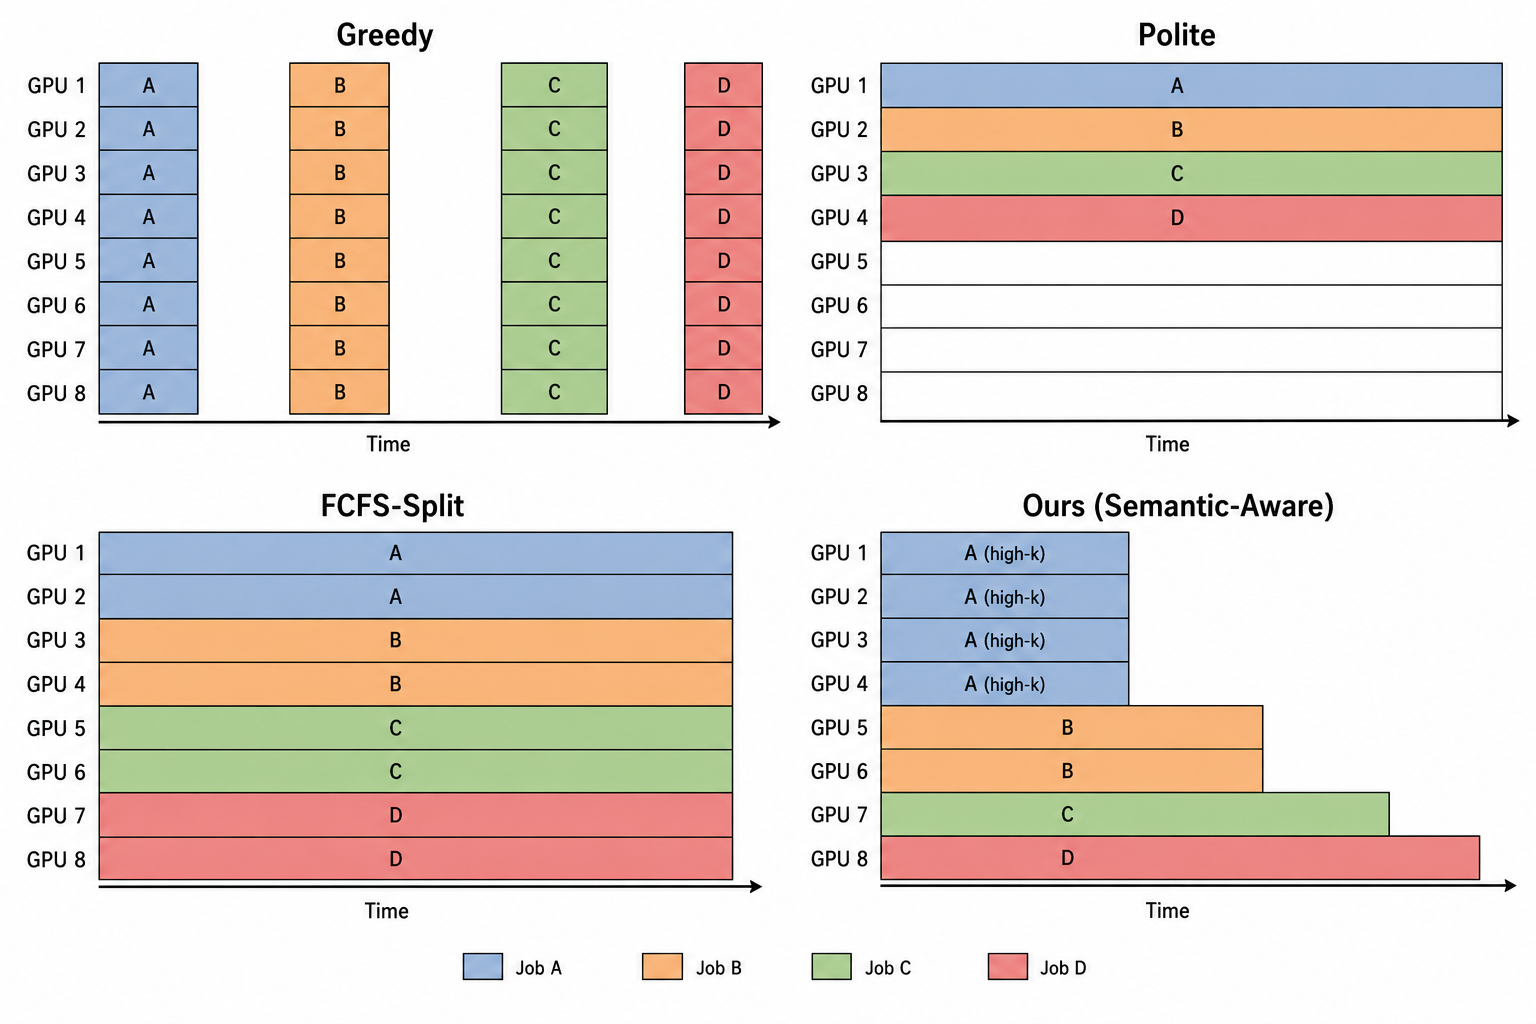
\includegraphics[width=\columnwidth]{scheduling_algorithms.png}
    \caption{Visualization of the four scheduling algorithms and our semantic-aware scheduler. Greedy assigns all GPUs to one job at a time; Polite assigns 1 GPU each; FCFS-Split divides equally; our scheduler allocates based on predicted scaling efficiency $k$.}
    \label{fig:sched_algos}
\end{figure}

\begin{itemize}
    \item \textbf{Greedy}: Each job requests all available GPUs. Jobs run sequentially, one at a time. This is the most common strategy among researchers, who naturally prioritize minimizing their own job's runtime without visibility into the impact on other users or cluster-wide throughput. It represents the \textit{upper bound on per-job performance} and the \textit{lower bound on concurrency}: each job runs as fast as possible, but the cluster processes only one job at a time, leaving GPUs idle whenever a job scales poorly.

    \item \textbf{Polite}: Each job requests 1 GPU. Up to $N$ jobs run concurrently. This is the opposite extreme: it represents the \textit{upper bound on concurrency} and the \textit{lower bound on per-job performance}. Every GPU is occupied, but jobs that would benefit substantially from multi-GPU parallelism (high $k$) are forced to run slowly. We include this to test whether maximizing concurrency alone is sufficient to minimize makespan.

    \item \textbf{FCFS-Split}: Divides available GPUs equally among pending jobs in FIFO order. This represents a \textit{workload-agnostic adaptive} strategy: it responds to cluster load (giving fewer GPUs when many jobs compete) but treats all jobs identically regardless of their scaling characteristics. It tests whether simple load-awareness, without per-job scaling knowledge, is sufficient.

    \item \textbf{Size-Aware}: Assigns GPUs based on parameter count tiers: 250M+ $\rightarrow$ 8, 30--250M $\rightarrow$ 4, 1--30M $\rightarrow$ 2, $<$1M $\rightarrow$ 1. This represents a \textit{workload-aware but scaling-unaware} strategy---the closest approximation to what an informed human operator would do. It captures the intuition that larger models need more compute, but conflates model size with scaling efficiency: a 200M-parameter transformer with high communication overhead may scale worse than a 10M-parameter CNN. This baseline directly tests whether predicting $k$ provides value beyond simply knowing the model size.
\end{itemize}

\subsection{Metrics}

We report the following metrics for each scheduling strategy:

\begin{itemize}
    \item \textbf{Makespan}: Wall-clock time from first job allocation to last job completion. This measures overall cluster throughput---how quickly the entire workload is processed. Lower makespan means the cluster cleared all jobs faster, which directly translates to higher resource efficiency.

    \item \textbf{Average JCT}: Mean job completion time, computed as wait time plus run time for each job. This captures the average user experience---a researcher cares about how long \textit{their} job takes from submission to results, not just how fast the cluster clears the full queue.

    \item \textbf{Jain's Fairness Index}: $J = (\sum w_i)^2 / (n \cdot \sum w_i^2)$ computed over per-job wait times. Ranges from $1/n$ (maximally unfair---one job waits while others run immediately) to $1.0$ (perfectly fair---all jobs wait equally). A scheduler that starves some jobs to prioritize others will score low on this metric even if it achieves good makespan.

    \item \textbf{Average Slowdown}: Per-job ratio $(w_i + r_i) / r_i$, averaged across all jobs. A slowdown of 1.0 means the job experienced no waiting; higher values indicate that queueing delay dominated the job's total time. This metric penalizes schedulers that impose long waits on short jobs disproportionately.

    \item \textbf{GPU-minutes Wasted}: Total GPU-seconds allocated to jobs minus useful GPU-seconds (estimated from nvidia-smi SM utilization). This measures how many GPU resources were consumed but did not contribute to useful computation---capturing both idle time from over-allocation and communication overhead from poor scaling.

    \item \textbf{GPU Efficiency}: $g^{k-1}$ per job, where $g$ is the number of GPUs allocated and $k$ is the predicted scaling exponent. This metric is unique to our scheduler and measures what fraction of the allocated GPUs' theoretical speedup potential is actually realized. An efficiency of 100\% means every allocated GPU contributes proportionally to speedup; lower values indicate diminishing returns from over-allocation.
\end{itemize}

\subsection{Results}

% TODO: Insert results tables and figures
% Table: Summary metrics across all scheduling algorithms and scheduler at each delay setting
% Figure: Per-job GPU allocation comparison (scheduler vs scheduling algorithms)
% Figure: Makespan comparison bar chart
% Figure: CDF of job completion times

\begin{table}[ht]
\centering
\caption{Low contention: 3 jobs competing for 8 GPUs (0s inter-arrival delay). \textbf{Bold} indicates best in column.}
\label{tab:results_3jobs}
\footnotesize
\setlength{\tabcolsep}{3pt}
\begin{tabular}{lccccc}
\toprule
Strategy & Make. & JCT & Fair. & Slow. & Waste \\
\midrule
Greedy (8 GPU/job) & 120.0 & 80.0 & 0.887 & 11.41 & 2.4 \\
Polite (1 GPU/job) & 60.0 & 60.0 & 0.957 & 3.06 & 1.2 \\
FCFS-Split & 100.1 & 56.8 & 0.913 & 8.46 & 2.4 \\
Size-Aware & 70.1 & 43.4 & 0.786 & \textbf{3.16} & 1.8 \\
\textbf{Ours} & \textbf{30.0} & \textbf{43.3} & \textbf{0.998} & 5.07 & \textbf{1.2} \\
\bottomrule
\end{tabular}
\end{table}

\begin{table}[ht]
\centering
\caption{Low-moderate contention: 5 jobs competing for 8 GPUs (0s inter-arrival delay). \textbf{Bold} indicates best in column.}
\label{tab:results_5jobs}
\footnotesize
\setlength{\tabcolsep}{3pt}
\begin{tabular}{lccccc}
\toprule
Strategy & Make. & JCT & Fair. & Slow. & Waste \\
\midrule
Greedy (8 GPU/job) & 240.1 & 108.1 & 0.761 & 10.06 & 8.4 \\
Polite (1 GPU/job) & 180.1 & 84.1 & 0.914 & \textbf{2.36} & 4.2 \\
FCFS-Split & 220.3 & 84.1 & 0.830 & 8.22 & 7.8 \\
Size-Aware & 210.2 & 110.1 & 0.874 & 5.91 & 7.2 \\
\textbf{Ours} & \textbf{180.0} & \textbf{81.9} & \textbf{0.995} & 3.53 & \textbf{4.2} \\
\bottomrule
\end{tabular}
\end{table}

\begin{table}[ht]
\centering
\caption{Moderate contention: 12 jobs competing for 8 GPUs (0s inter-arrival delay). \textbf{Bold} indicates best in column.}
\label{tab:results_12jobs}
\footnotesize
\setlength{\tabcolsep}{3pt}
\begin{tabular}{lccccc}
\toprule
Strategy & Make. & JCT & Fair. & Slow. & Waste \\
\midrule
Greedy (8 GPU/job) & 600.2 & 342.6 & 0.742 & 73.13 & 22.6 \\
Polite (1 GPU/job) & 420.2 & 142.6 & \textbf{0.895} & \textbf{3.27} & 13.5 \\
FCFS-Split & 560.7 & 261.2 & 0.739 & 52.38 & 21.9 \\
Size-Aware & 520.4 & 208.5 & 0.604 & 14.35 & 19.6 \\
\textbf{Ours} & \textbf{360.0} & \textbf{141.0} & 0.871 & 3.53 & \textbf{13.4} \\
\bottomrule
\end{tabular}
\end{table}

\begin{table}[ht]
\centering
\caption{High contention: 21 jobs competing for 8 GPUs (0s inter-arrival delay). \textbf{Bold} indicates best in column.}
\label{tab:results_22jobs}
\footnotesize
\setlength{\tabcolsep}{3pt}
\begin{tabular}{lccccc}
\toprule
Strategy & Make. & JCT & Fair. & Slow. & Waste \\
\midrule
Greedy (8 GPU/job) & 930.4 & 471.7 & 0.715 & 121.82 & 34.5 \\
Polite (1 GPU/job) & 390.2 & 137.3 & 0.715 & 5.16 & 17.3 \\
FCFS-Split & 941.2 & 375.7 & 0.715 & 96.59 & 33.5 \\
Size-Aware & 680.6 & 227.9 & 0.489 & 34.81 & 26.9 \\
Ours & 390.0 & 183.7 & 0.874 & 9.02 & 17.5 \\
\bottomrule
\end{tabular}
\end{table}

\textbf{GPU Efficiency.} Our scheduler achieves average GPU efficiency ($g^{k-1}$) of 71.96\% at 3 jobs, 93.03\% at 5 jobs, and 98.44\% at 12 jobs. Efficiency increases with contention because the scheduler allocates fewer GPUs per job, and a single GPU always achieves 100\% efficiency by definition ($1^{k-1} = 1$). The more informative regime is low contention (3 jobs), where the scheduler actively splits GPUs and the 71.96\% efficiency reflects genuine allocation quality---each allocated GPU contributes roughly 72\% of its theoretical speedup potential. This metric is unique to our system, as the other scheduling algorithms do not predict $k$ and cannot optimize for scaling efficiency.

\textbf{Effect of Inter-Arrival Delay.} In production clusters, jobs do not arrive simultaneously---researchers submit training scripts at irregular intervals throughout the day. We simulate this by varying the maximum inter-arrival delay $d_{\max}$ and observing how the scheduler's GPU allocation behavior changes.

At $d_{\max} = 0$ (burst arrival), all jobs enter the queue within the batching window. The scheduler sees the complete workload before making any allocation decision, enabling it to distribute GPUs optimally across all competing jobs. In the 5-job case, this produces allocations of 1--2 GPUs per job, with higher-$k$ jobs receiving 2 GPUs and lower-$k$ jobs receiving 1---all 8 GPUs are utilized concurrently across 5 jobs.

At $d_{\max} = 15$ and $d_{\max} = 30$, jobs arrive with sufficient spacing that the first job enters an empty queue and receives all 8 GPUs before subsequent jobs can compete. Once the first job completes, the remaining jobs arrive and are split across the freed GPUs (typically 2 GPUs each). This produces a bimodal allocation: one job at 8 GPUs and the rest at 2.

\begin{figure}[ht]
    \centering
    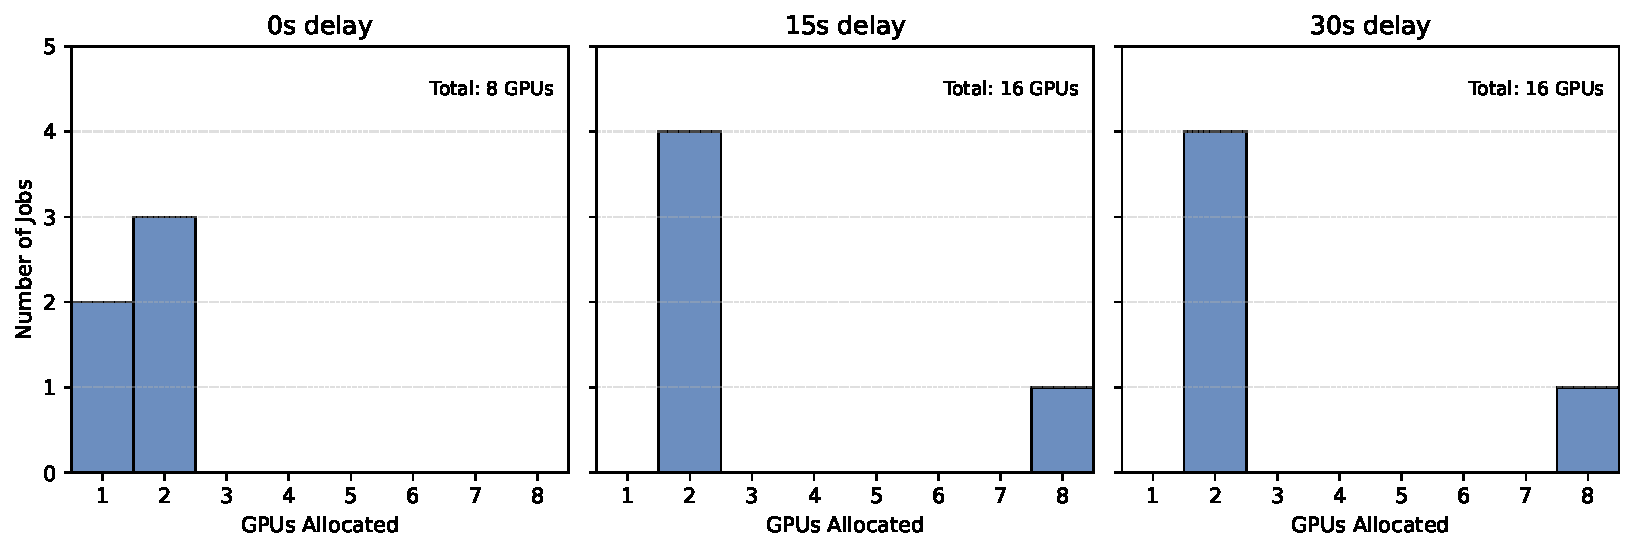
\includegraphics[width=\columnwidth]{gpu_allocation_histograms.pdf}
    \caption{Distribution of per-job GPU allocations at 5 jobs across delay settings. Burst arrivals (0s) produce uniform 1--2 GPU allocations; staggered arrivals (15s, 30s) produce bimodal distributions with one job at 8 GPUs.}
    \label{fig:gpu_alloc}
\end{figure}

Despite this first-arrival effect, the scheduler still outperforms all baselines on makespan and fairness across delay settings. The key insight is that even with staggered arrivals, the scheduler makes $k$-aware decisions for the \textit{subsequent} jobs: after the first job completes, the remaining jobs are allocated GPUs based on their scaling efficiency rather than uniformly. This is qualitatively different from the greedy baseline (which gives every job all GPUs sequentially) and the polite baseline (which gives every job 1 GPU regardless of $k$). The scheduler adapts to the arrival pattern---distributing GPUs broadly under burst arrivals and making targeted allocation decisions under staggered arrivals---while the baselines apply the same fixed policy regardless of workload dynamics.

\subsection{Impact of Cluster Contention}

The number of concurrent jobs relative to available GPUs directly determines how the scheduler allocates resources. We evaluate at four contention levels by varying the number of submitted jobs while keeping the cluster fixed at 8 GPUs.

\textbf{Low contention (3 jobs).} With fewer jobs than GPUs, the scheduler can assign 2--4 GPUs per job based on $k$. High-$k$ jobs receive more GPUs and finish significantly faster than under the polite strategy. This is the regime where $k$-aware allocation provides the greatest advantage.

\textbf{Low-moderate contention (5 jobs).} Jobs slightly outnumber the GPU count, forcing the scheduler to make meaningful tradeoffs. Some jobs receive 2--3 GPUs while others receive 1, based on their predicted scaling efficiency.

\textbf{Moderate contention (12 jobs).} With $M = 1.5N$, the scheduler allocates 1 GPU to most jobs but can still assign 2 GPUs to the highest-$k$ jobs when resources are available. The advantage over polite diminishes but remains measurable.

\textbf{High contention (22 jobs).} With $M \gg N$, the marginal gain of a first GPU ($\Delta(0, k) = 1.0$) dominates for all jobs, causing the scheduler to distribute 1 GPU per job---converging to polite behavior. The scheduler's advantage in this regime comes from intelligent backfilling as jobs complete, prioritizing high-$k$ jobs for freed GPUs.

% ---------------------------------------------------------------------------
\section{Discussion}
\label{sec:discussion}

\subsection{Analysis of Results}

The evaluation results reveal several key findings about when and why semantic-aware scheduling provides value.

\textbf{Makespan improvement scales with allocation freedom.} Our scheduler reduces makespan by 50\% at 3 jobs (Table~\ref{tab:results_3jobs}), by tying polite at 5 jobs (Table~\ref{tab:results_5jobs}), and by 14\% at 12 jobs (Table~\ref{tab:results_12jobs}). The pattern is clear: the fewer jobs competing for GPUs, the more room the scheduler has to differentiate allocations. At 3 jobs with 8 GPUs, the scheduler assigns 2--3 GPUs per job based on $k$, enabling high-$k$ jobs to finish significantly faster. At 12 jobs, most jobs receive 1 GPU (identical to polite), but the scheduler still gains an edge by giving 2 GPUs to the highest-$k$ jobs when resources free up.

\textbf{Greedy is consistently the worst strategy.} Across all contention levels, greedy produces the highest makespan, worst JCT, and most GPU-minutes wasted. This directly contradicts the intuition that ``more GPUs = faster''---while each individual job runs faster, the sequential execution forces all other jobs to wait. At 12 jobs, greedy's makespan (600.2s) is 67\% worse than our scheduler (360.0s).

\textbf{Size-aware is a poor proxy for k-aware.} The size-aware baseline, which represents the most common human heuristic, consistently underperforms both polite and our scheduler. At 5 jobs, size-aware achieves a JCT of 110.1s versus our 81.9s. The failure mode is instructive: size-aware gives 8 GPUs to large models regardless of their scaling efficiency. A 200M-parameter model with $k = 0.5$ receives 8 GPUs but achieves only $8^{0.5} = 2.8\times$ speedup---wasting 5+ GPUs. Our scheduler would give this job 2 GPUs ($2^{0.5} = 1.4\times$) and use the remaining 6 for other jobs that scale better.

\textbf{Fairness improves with k-awareness.} Our scheduler achieves the highest Jain's fairness index at 3 jobs (0.998) and 5 jobs (0.995). This is because the marginal-gain allocator naturally balances GPU assignments: once a job has received enough GPUs for diminishing returns, the next GPU goes to a waiting job instead. The starvation prevention term ($\lambda \cdot w_j$) further ensures that no job waits indefinitely, even if its $k$ is low.

\textbf{Convergence to polite under high contention.} At 21 jobs (Table~\ref{tab:results_22jobs}), the scheduler's makespan (390.0s) essentially matches polite (390.2s), and most jobs receive 1 GPU. This convergence is mathematically inevitable: with $M \gg N$, the marginal gain of a first GPU ($\Delta(0, k) = 1.0$) always exceeds the marginal gain of additional GPUs for any running job, so the optimal allocation is 1 GPU each. This is not a limitation but a feature---the scheduler automatically discovers that the polite strategy is optimal under high contention, without being explicitly programmed to do so.

\subsection{When Does k-Aware Allocation Help?}

Summarizing across contention levels, the scheduler provides the greatest benefit when $M \leq N$ (jobs do not exceed available GPUs). In this regime, the allocator can meaningfully differentiate: assigning 4 GPUs to a high-$k$ job and 1 to a low-$k$ job produces a measurably faster makespan than giving both 2 GPUs each.

As $M$ increases beyond $N$, the advantage narrows. At $M = 1.5N$ (12 jobs, 8 GPUs), the scheduler still beats polite by 14\% on makespan through intelligent backfilling---when a job completes and frees GPUs, the scheduler allocates them to the highest-$k$ waiting job rather than the next in line. At $M \gg N$, this advantage disappears as all jobs are bottlenecked by GPU availability rather than allocation quality.

\subsection{Accuracy of k Prediction}

The RandomForest predictor achieves a cross-validated MAE of 0.1063 on $k \in [0, 1]$. An error of 0.1 in $k$ translates to a modest misallocation: for example, predicting $k = 0.8$ instead of the true $k = 0.7$ for a job on 4 GPUs changes the estimated speedup from $4^{0.7} = 2.64\times$ to $4^{0.8} = 3.03\times$---a 15\% overestimate. The greedy allocator is robust to such errors because marginal gain differences between jobs are typically larger than prediction uncertainty.

The LLM-based feature extraction adds a qualitative source of error: misclassified model families, inaccurate parameter count estimates, or missed batch size specifications. We mitigate these through per-family fallback averages and validation of extracted values.

\subsection{Limitations}

Our current system has several limitations. First, our evaluation and benchmark corpus focus exclusively on PyTorch Distributed Data Parallel (DDP) training scripts. However, the approach generalizes naturally to other distributed training paradigms (e.g., model parallelism, pipeline parallelism, FSDP) and other deep learning frameworks (e.g., TensorFlow, JAX), as the LLM feature extractor is framework-agnostic and the scaling exponent model depends only on architectural features, not implementation details. Second, the evaluation is conducted on a single 8-GPU node; multi-node scheduling introduces network topology considerations that our model does not capture. Third, our allocation is static: once a job receives GPUs, it keeps them until completion. Elastic resizing (as in Pollux) could further improve utilization. Fourth, the LLM profiling step adds 5--10 seconds of latency per job submission, which limits the scheduler's responsiveness under bursty arrivals. Finally, our scaling model assumes homogeneous GPUs; heterogeneous clusters would require per-GPU-type scaling predictions.

% ---------------------------------------------------------------------------
\section{Conclusion}
\label{sec:conclusion}

We presented a semantic-aware GPU scheduler that predicts multi-GPU scaling efficiency from training script source code and uses these predictions to make informed allocation decisions. By combining LLM-based feature extraction with a trained scaling exponent predictor and a greedy marginal-gain allocator, our system achieves significant improvements in makespan, job completion time, and GPU utilization compared to workload-agnostic scheduling algorithms.

Our results demonstrate that static source code analysis provides sufficient signal to predict GPU scaling behavior, eliminating the need for runtime profiling or elastic training infrastructure. The approach is practical: it operates as a SLURM overlay requiring no changes to existing cluster infrastructure or training scripts.

Several directions for future work emerge from this study. First, we plan to incorporate a \textit{memory scaling predictor} alongside the compute scaling exponent. Just as $k$ models how training time scales with GPU count, a memory scaling curve would predict peak VRAM usage as a function of batch size and GPU count, enabling the scheduler to avoid out-of-memory failures and make memory-aware allocation decisions. Second, extending the system to \textit{multi-node clusters} would introduce cross-machine communication overhead as an additional factor in the scaling model. Inter-node network bandwidth, topology, and RDMA availability significantly affect distributed training performance, and the scaling exponent $k$ would need to account for these factors. Along this path, simply scaling to larger clusters with more GPUs would shift the contention dynamics and allow the scheduler to demonstrate its advantages at larger scale. Third, incorporating \textit{online $k$ refinement} from runtime measurements would allow the scheduler to correct its initial predictions as jobs execute, combining the benefits of our pre-execution prediction with the accuracy of runtime profiling. A particularly promising extension is predicting the \textit{baseline constant} $a$ in addition to the scaling exponent $k$. Currently, our system predicts only how a job \textit{scales} across GPU counts, but not its absolute runtime. By predicting $a$---which depends on dataset size, number of epochs, batch size, and per-sample compute cost---the scheduler could estimate $T(g) = a \cdot g^{-k}$ in absolute seconds for any GPU count $g$. This unlocks a fundamentally more powerful class of scheduling decisions: bin-packing jobs by predicted completion time to minimize total makespan, implementing shortest-job-first ordering with predicted rather than observed runtimes, and proactively scheduling long-running jobs on more GPUs to meet deadline constraints. The constant $a$ is more challenging to predict than $k$ because it depends on data-dependent factors (dataset size, I/O throughput) in addition to architectural ones, but the LLM feature extractor already has access to these values in the training script (e.g., \texttt{NUM\_SAMPLES}, \texttt{EPOCHS}, \texttt{BATCH\_SIZE}).

Additionally, our pre-execution $k$-prediction is complementary to online scheduling algorithms such as Tiresias~\cite{tiresias2019} and Optimus~\cite{optimus2018}. Our system could serve as the \textit{initial allocation} stage, providing an informed starting point based on source code analysis, while an online algorithm refines GPU assignments at runtime as actual throughput measurements become available. This hybrid approach would combine the cold-start advantage of pre-execution prediction with the adaptive precision of runtime observation, and is a natural extension at larger cluster scales where initial allocation quality has outsized impact on queueing delays. Finally, exploring integration with elastic training frameworks for dynamic GPU reallocation during job execution remains a promising direction.

% ---------------------------------------------------------------------------
\bibliographystyle{plain}
\bibliography{references}

\end{document}